\documentclass{beamer}
\usepackage{pdfpages}
%Imports and customization
\usepackage{tikz}
\usepackage{graphicx}
\usepackage{tikz-feynman}
\usepackage{ulem}
\usepackage{colortbl}
\graphicspath{ 
    {./images/}
}

\beamertemplatenavigationsymbolsempty
\setbeamertemplate{sidebar right}{}
\setbeamertemplate{footline}{
    \hfill\usebeamertemplate***{navigation symbols}
    \hspace{1cm}\insertframenumber{}/\inserttotalframenumber
}
\setbeamertemplate{caption}{\raggedright\insertcaption\par}
\setbeamersize{text margin left=4mm,text margin right=4mm} 

\setbeamerfont{itemize/enumerate body}{size=\scriptsize}
\setbeamerfont{itemize/enumerate subbody}{size=\scriptsize}
\setbeamerfont{itemize/enumerate subsubbody}{size=\scriptsize}


%Custom Macros
\newcommand{\statwarn}{
    \tiny \color{red} Absolute numbers here mean NOTHING. Plots are based on small (100k events) samples, and are highly biased. All that matters is relative position!
}


% WARNING: When using these commands, the image argument must
% NOT have spaces between itself and the braces
\newcommand{\fullscreenimage}[2]{
    \frame{
        \frametitle{#1} 
        \begin{figure}
        \includegraphics[height=0.9\textheight,width=\textwidth,keepaspectratio]{#2}
        \end{figure}
    }
}


\newcommand{\importpdf}[3]{
    \frame{
        \begin{columns}\column{\dimexpr\paperwidth-10pt}
        \begin{figure}
        \includegraphics[page=#2,height=0.8\textheight,width=\textwidth,keepaspectratio]{#1}
        \end{figure}

        {\tiny #3}
        \end{columns}
    }
}


\newcommand{\displayone}[3]{
    \frame{
        \frametitle{#1} 
        \begin{columns}
            \begin{column}{0.5\textwidth}
                #2
            \end{column}
            \begin{column}{0.5\textwidth}
                \begin{figure}
                    \includegraphics[width=\linewidth,height=\textheight,keepaspectratio]{#3}
                \end{figure}
            \end{column}
        \end{columns}
    }
}

\newcommand{\displayonelarge}[3]{
    \frame{
        \frametitle{#1} 
        \begin{columns}
            \begin{column}{0.3\textwidth}
                #2
            \end{column}
            \begin{column}{0.7\textwidth}
                \begin{figure}
                    \includegraphics[width=\linewidth,height=0.8\textheight,keepaspectratio]{#3}
                \end{figure}
            \end{column}
        \end{columns}
    }
}


\newcommand{\displaytwo}[4]{
    \frame{
        \frametitle{#1} 
        #2
        \begin{columns}
            \begin{column}{0.5\textwidth}
                \begin{figure}
                    \includegraphics[width=\linewidth,height=\textheight,keepaspectratio]{#3}
                \end{figure}
            \end{column}
            \begin{column}{0.5\textwidth}
                \begin{figure}
                    \includegraphics[width=\linewidth,height=\textheight,keepaspectratio]{#4}
                \end{figure}
            \end{column}
        \end{columns}
    }
}

\newcommand{\displaytwocaption}[6]{
    \frame{
        \frametitle{#1} 
        #2
        \begin{columns}
            \begin{column}{0.5\textwidth}
                \begin{figure}
                    \includegraphics[width=\linewidth,height=\textheight,keepaspectratio]{#3}
                    \caption{#4}
                \end{figure}
            \end{column}
            \begin{column}{0.5\textwidth}
                \begin{figure}
                    \includegraphics[width=\linewidth,height=\textheight,keepaspectratio]{#5}
                    \caption{#6}
                \end{figure}
            \end{column}
        \end{columns}
    }
}

\newcommand{\displaytwoVcaption}[6]{
    \frame{
        \begin{columns}
            \begin{column}{0.5\textwidth}
                \frametitle{#1} 
                #2
            \end{column}
            \begin{column}{0.5\textwidth}
                \begin{figure}
                    \includegraphics[width=\linewidth,height=0.3\textheight,keepaspectratio]{#3}
                    \caption{#4}
                \end{figure}

                \begin{figure}
                    \includegraphics[width=\linewidth,height=0.3\textheight,keepaspectratio]{#5}
                    \caption{#6}
                \end{figure}
            \end{column}
        \end{columns}
    }
}


\newcommand{\displaythree}[5]{
    \frame{
        \begin{columns}[T]
            \begin{column}{0.4\textwidth}
                {\usebeamercolor[fg]{title} \insertframetitle{#1} }\\
                \vspace{5mm}
                #2
            \end{column}
            \begin{column}{0.4\textwidth}
                \begin{figure}
                    \includegraphics[width=\linewidth,height=\textheight,keepaspectratio]{#3}
                \end{figure}
            \end{column}
        \end{columns}
        \begin{columns}[T]
            \begin{column}{0.4\textwidth}
                \begin{figure}
                    \includegraphics[width=\linewidth,height=\textheight,keepaspectratio]{#4}
                \end{figure}
            \end{column}
            \begin{column}{0.4\textwidth}
                \begin{figure}
                    \includegraphics[width=\linewidth,height=\textheight,keepaspectratio]{#5}
                \end{figure}
            \end{column}
        \end{columns}
    }
}


\newcommand{\displayfour}[5]{
    \frame{
        \frametitle{#1} 
        \begin{columns}[T]
            \begin{column}{0.4\textwidth}
                \begin{figure}
                    \includegraphics[width=\linewidth,height=\textheight,keepaspectratio]{#2}
                \end{figure}
            \end{column}
            \begin{column}{0.4\textwidth}
                \begin{figure}
                    \includegraphics[width=\linewidth,height=\textheight,keepaspectratio]{#3}
                \end{figure}
            \end{column}
        \end{columns}
        \begin{columns}[T]
            \begin{column}{0.4\textwidth}
                \begin{figure}
                    \includegraphics[width=\linewidth,height=\textheight,keepaspectratio]{#4}
                \end{figure}
            \end{column}
            \begin{column}{0.4\textwidth}
                \begin{figure}
                    \includegraphics[width=\linewidth,height=\textheight,keepaspectratio]{#5}
                \end{figure}
            \end{column}
        \end{columns}
    }
}


\newcommand{\pstrike}[2]{
    \only<-\the\numexpr#1-1>{#2}
    \only<#1->{\sout{#2}}
}


\newcommand{\announcesection}[1]{
    \section{#1}
    \frame{
        \begin{center}
            {\huge #1} 
        \end{center}
    }
}

\newcommand{\kvv}{\kappa_{2V}}
\newcommand{\kl}{\kappa_{\lambda}}
\newcommand{\kv}{\kappa_{V}}

\newcommand{\fkvv}[1]{\kappa_{2V,#1}}
\newcommand{\fkl} [1]{\kappa_{\lambda,#1}}
\newcommand{\fkv} [1]{\kappa_{V,#1}}

\newcommand{\importpdfwpages}[3]{
    \foreach \pageN in {#2,...,#3}{
        \importpdf{#1}{\pageN}{}
    }
}

\newcommand{\hyper}[2]{{\color{blue}\href{#1}{#2}}}



%Begin Presentation
\begin{document}
    \setbeamercolor{background canvas}{bg=}
    \title{Updates on VBF HH Coupling Scans}
    \author{Chris Milke}
    \date{16 March, 2021}

    \frame{\titlepage}

    %\frame{\frametitle{Overview} \tableofcontents}
    % last time
    \announcesection{Last Time, Truth Reweighting}
    \importpdfwpages{last_time}{1}{4}

    % 2D reweighting
    \section{Reweighting with Two Variables}

\displayonelarge{Reweighting with Two Variables} {
        Attempted 2D reweighting using all 21 combinations of the following 7 kinematic variables:
        \vspace{10mm}
        \begin{itemize} {
            {\large \item $M_{hh}$ }
            {\large \item $\Delta \eta_{hh}$ }
            {\large \item $p_{T,hh}$ }
            {\large \item $M_{jj}$ }
            {\large \item $\Delta \eta_{jj}$ }
            {\large \item $p_{T,jj}$ }
            {\large \item $p_{T}$ Sum, jj }
        } \end{itemize}
}{comb_mhh-mjj}



\frame{
    \frametitle{None of the 21 Combinations are Viable}
    Out of the 21 combinations of the 7 most obvious variables, none are even close to being usable for reweighting.

    \vspace{5mm}
    Note that this study is not exhaustive, and there are countless other variables and combinations of variables that could potentially show success.

    \vspace{5mm}
    However, finding the exact specific combination of variables could prove quite time-consuming, assuming such a combination even exists.
    As such, I am putting further research into VBF Reweighting on hold, and will focus efforts instead on direct linear combination of reconstructed, post-selection samples.

    \vspace{5mm}
    The direct combination approach has already proven useful for VBF, and focused effort could further improve it.
}


    % back to combinations, truth first, then reco
    \section{NNT Linear Combinations}

\frame{
    \frametitle{Linear Combination Using Full-Reco, Post-Selection Samples}
    \begin{columns}
        \begin{column}{0.4\textwidth}
            \begin{center} 
            {\tiny NNT Basis Set}

            \resizebox{0.2\textheight}{!}{ \begin{tabular}{ |l|l|l| }
                \hline
                \textbf {$\kappa_{2V}$} & \textbf {$\kappa_\lambda$} & \textbf {$\kappa_V$} \\
                \hline
                    1.  &   1. & 1.  \\
                    2.  &   1. & 1.  \\
                    1.5 &   1. & 1.  \\
                    0.  &   1. & 0.5 \\
                    1.  &   0. & 1.  \\
                    1.  &  10. & 1.  \\
                \hline
            \end{tabular}}
            \end{center}

        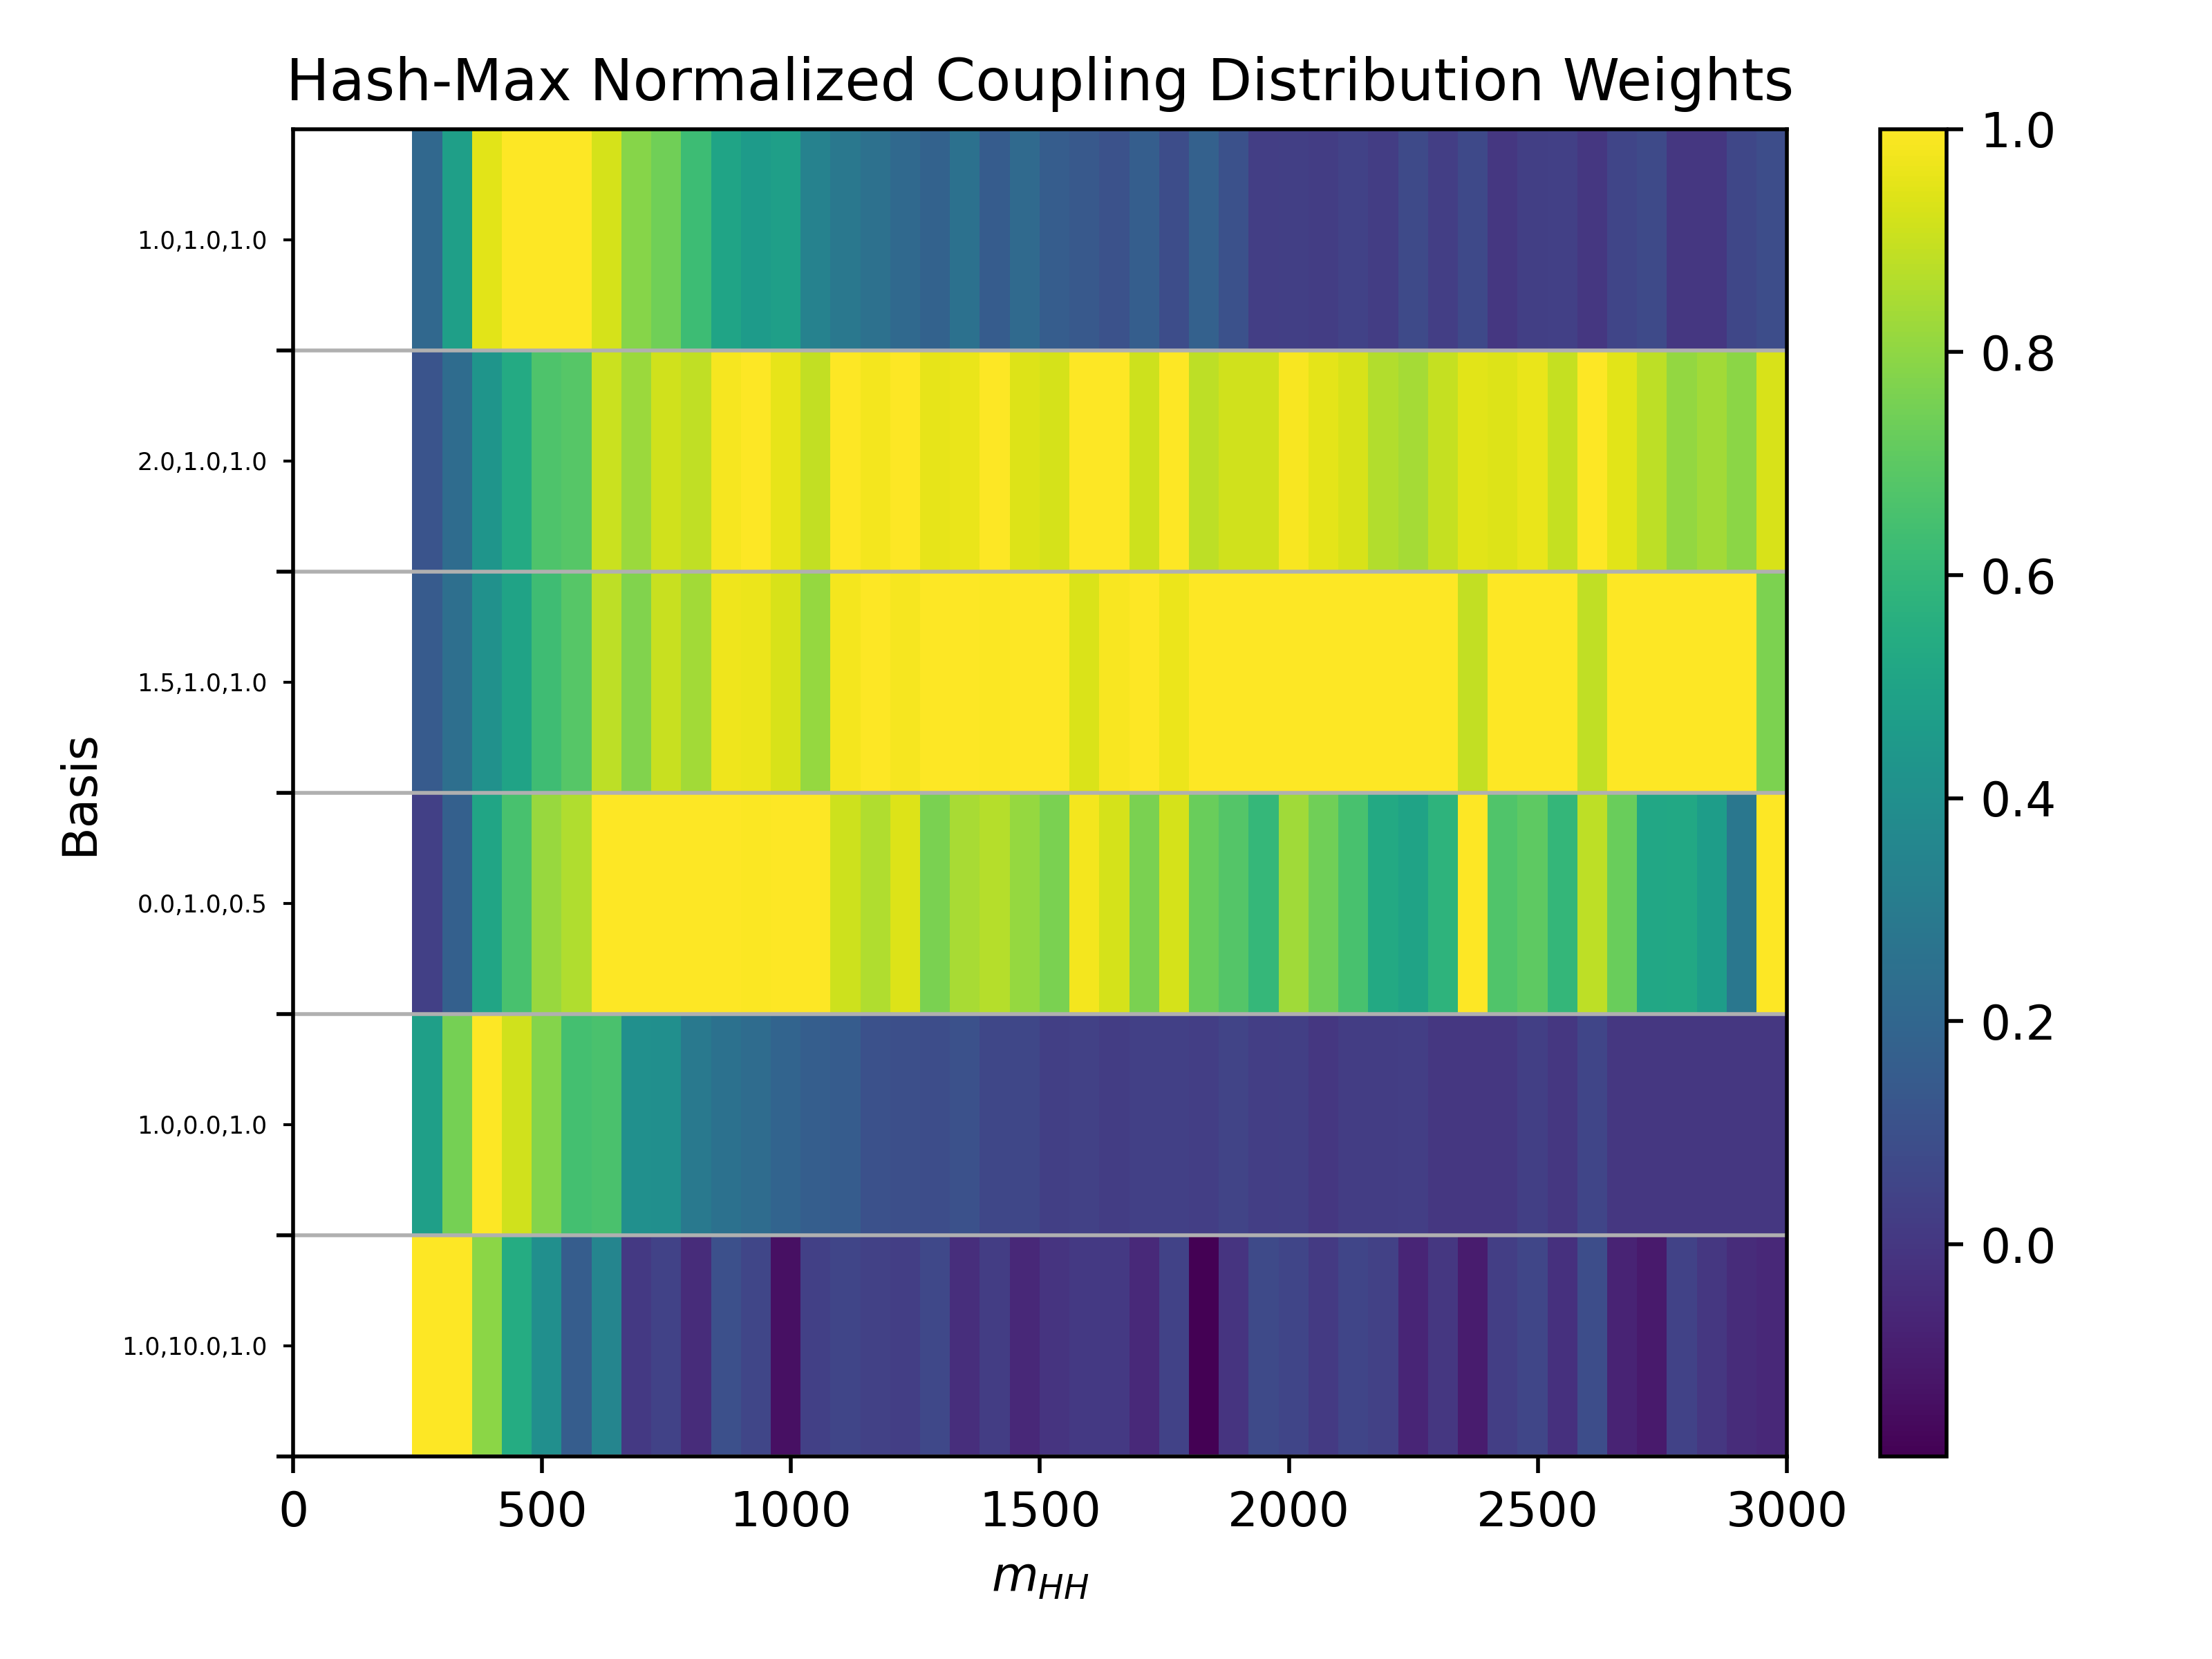
\includegraphics[width=\linewidth,height=\textheight,keepaspectratio]
            {coupling_scan_auto_chosen_reco_R0_hash_max}

        \end{column}
        \begin{column}{0.6\textwidth}
            \resizebox{0.8\textwidth}{!}{ \begin{minipage}{1.0\textwidth}
            Linear Combination Equation

            \vspace{10mm}

            {\tiny $
    \left(2 \kappa_{2V}^{2} - \frac{124 \kappa_{2V} \kappa_{V}^{2}}{9} + \frac{61 \kappa_{2V} \kappa_{V} \kappa_{\lambda}}{9} + \frac{106 \kappa_{V}^{4}}{9} - \frac{17 \kappa_{V}^{3} \kappa_{\lambda}}{3} - \frac{\kappa_{V}^{2} \kappa_{\lambda}^{2}}{9}\right) \left|{A{\left(1,1,1 \right)}}\right|^{2} +
$

$
    \left(2 \kappa_{2V}^{2} - 8 \kappa_{2V} \kappa_{V}^{2} + 3 \kappa_{2V} \kappa_{V} \kappa_{\lambda} + 6 \kappa_{V}^{4} - 3 \kappa_{V}^{3} \kappa_{\lambda}\right) \left|{A{\left(2,1,1 \right)}}\right|^{2} +
$

$
    \left(- 4 \kappa_{2V}^{2} + 20 \kappa_{2V} \kappa_{V}^{2} - 8 \kappa_{2V} \kappa_{V} \kappa_{\lambda} - 16 \kappa_{V}^{4} + 8 \kappa_{V}^{3} \kappa_{\lambda}\right) \left|{A{\left(1.5,1,1 \right)}}\right|^{2} +
$

$
    \left(16 \kappa_{2V} \kappa_{V}^{2} - 16 \kappa_{2V} \kappa_{V} \kappa_{\lambda} - 16 \kappa_{V}^{4} + 16 \kappa_{V}^{3} \kappa_{\lambda}\right) \left|{A{\left(0,1,0.5 \right)}}\right|^{2} +
$

$
    \left(\frac{4 \kappa_{2V} \kappa_{V}^{2}}{5} - \frac{4 \kappa_{2V} \kappa_{V} \kappa_{\lambda}}{5} + \frac{\kappa_{V}^{4}}{5} - \frac{3 \kappa_{V}^{3} \kappa_{\lambda}}{10} + \frac{\kappa_{V}^{2} \kappa_{\lambda}^{2}}{10}\right) \left|{A{\left(1,0,1 \right)}}\right|^{2} +
$

$
    \left(- \frac{\kappa_{2V} \kappa_{V}^{2}}{45} + \frac{\kappa_{2V} \kappa_{V} \kappa_{\lambda}}{45} + \frac{\kappa_{V}^{4}}{45} - \frac{\kappa_{V}^{3} \kappa_{\lambda}}{30} + \frac{\kappa_{V}^{2} \kappa_{\lambda}^{2}}{90}\right) \left|{A{\left(1,10,1 \right)}}\right|^{2}
$
}
            \end{minipage}}
        \end{column}
    \end{columns}
}

\displaythree{Validity of NNT Reweighting}
{ \small 
    Direct combination results are not optimal, but unlike truth reweighting they are usable.

    \vspace{2mm}
    Furthermore, there are a number of ideas to improve upon them that I will investigate in the coming weeks.
}
{reco_mHH_cvv1p0cl2p0cv1p0}
{reco_mHH_cvv0p0cl1p0cv1p0}
{reco_mHH_cvv4p0cl1p0cv1p0}


    \frame{
    \frametitle{Coupling Interpolation Through NNT Direct Combination}
    \begin{columns}
        \begin{column}{0.4\textwidth}
            \begin{center} 
            {\tiny NNT Basis Set}

            \resizebox{0.2\textheight}{!}{ \begin{tabular}{ |l|l|l| }
                \hline
                \textbf {$\kappa_{2V}$} & \textbf {$\kappa_\lambda$} & \textbf {$\kappa_V$} \\
                \hline
                    1.  &   1. & 1.  \\
                    2.  &   1. & 1.  \\
                    1.5 &   1. & 1.  \\
                    0.  &   1. & 0.5 \\
                    1.  &   0. & 1.  \\
                    1.  &  10. & 1.  \\
                \hline
            \end{tabular}}
            \end{center}

        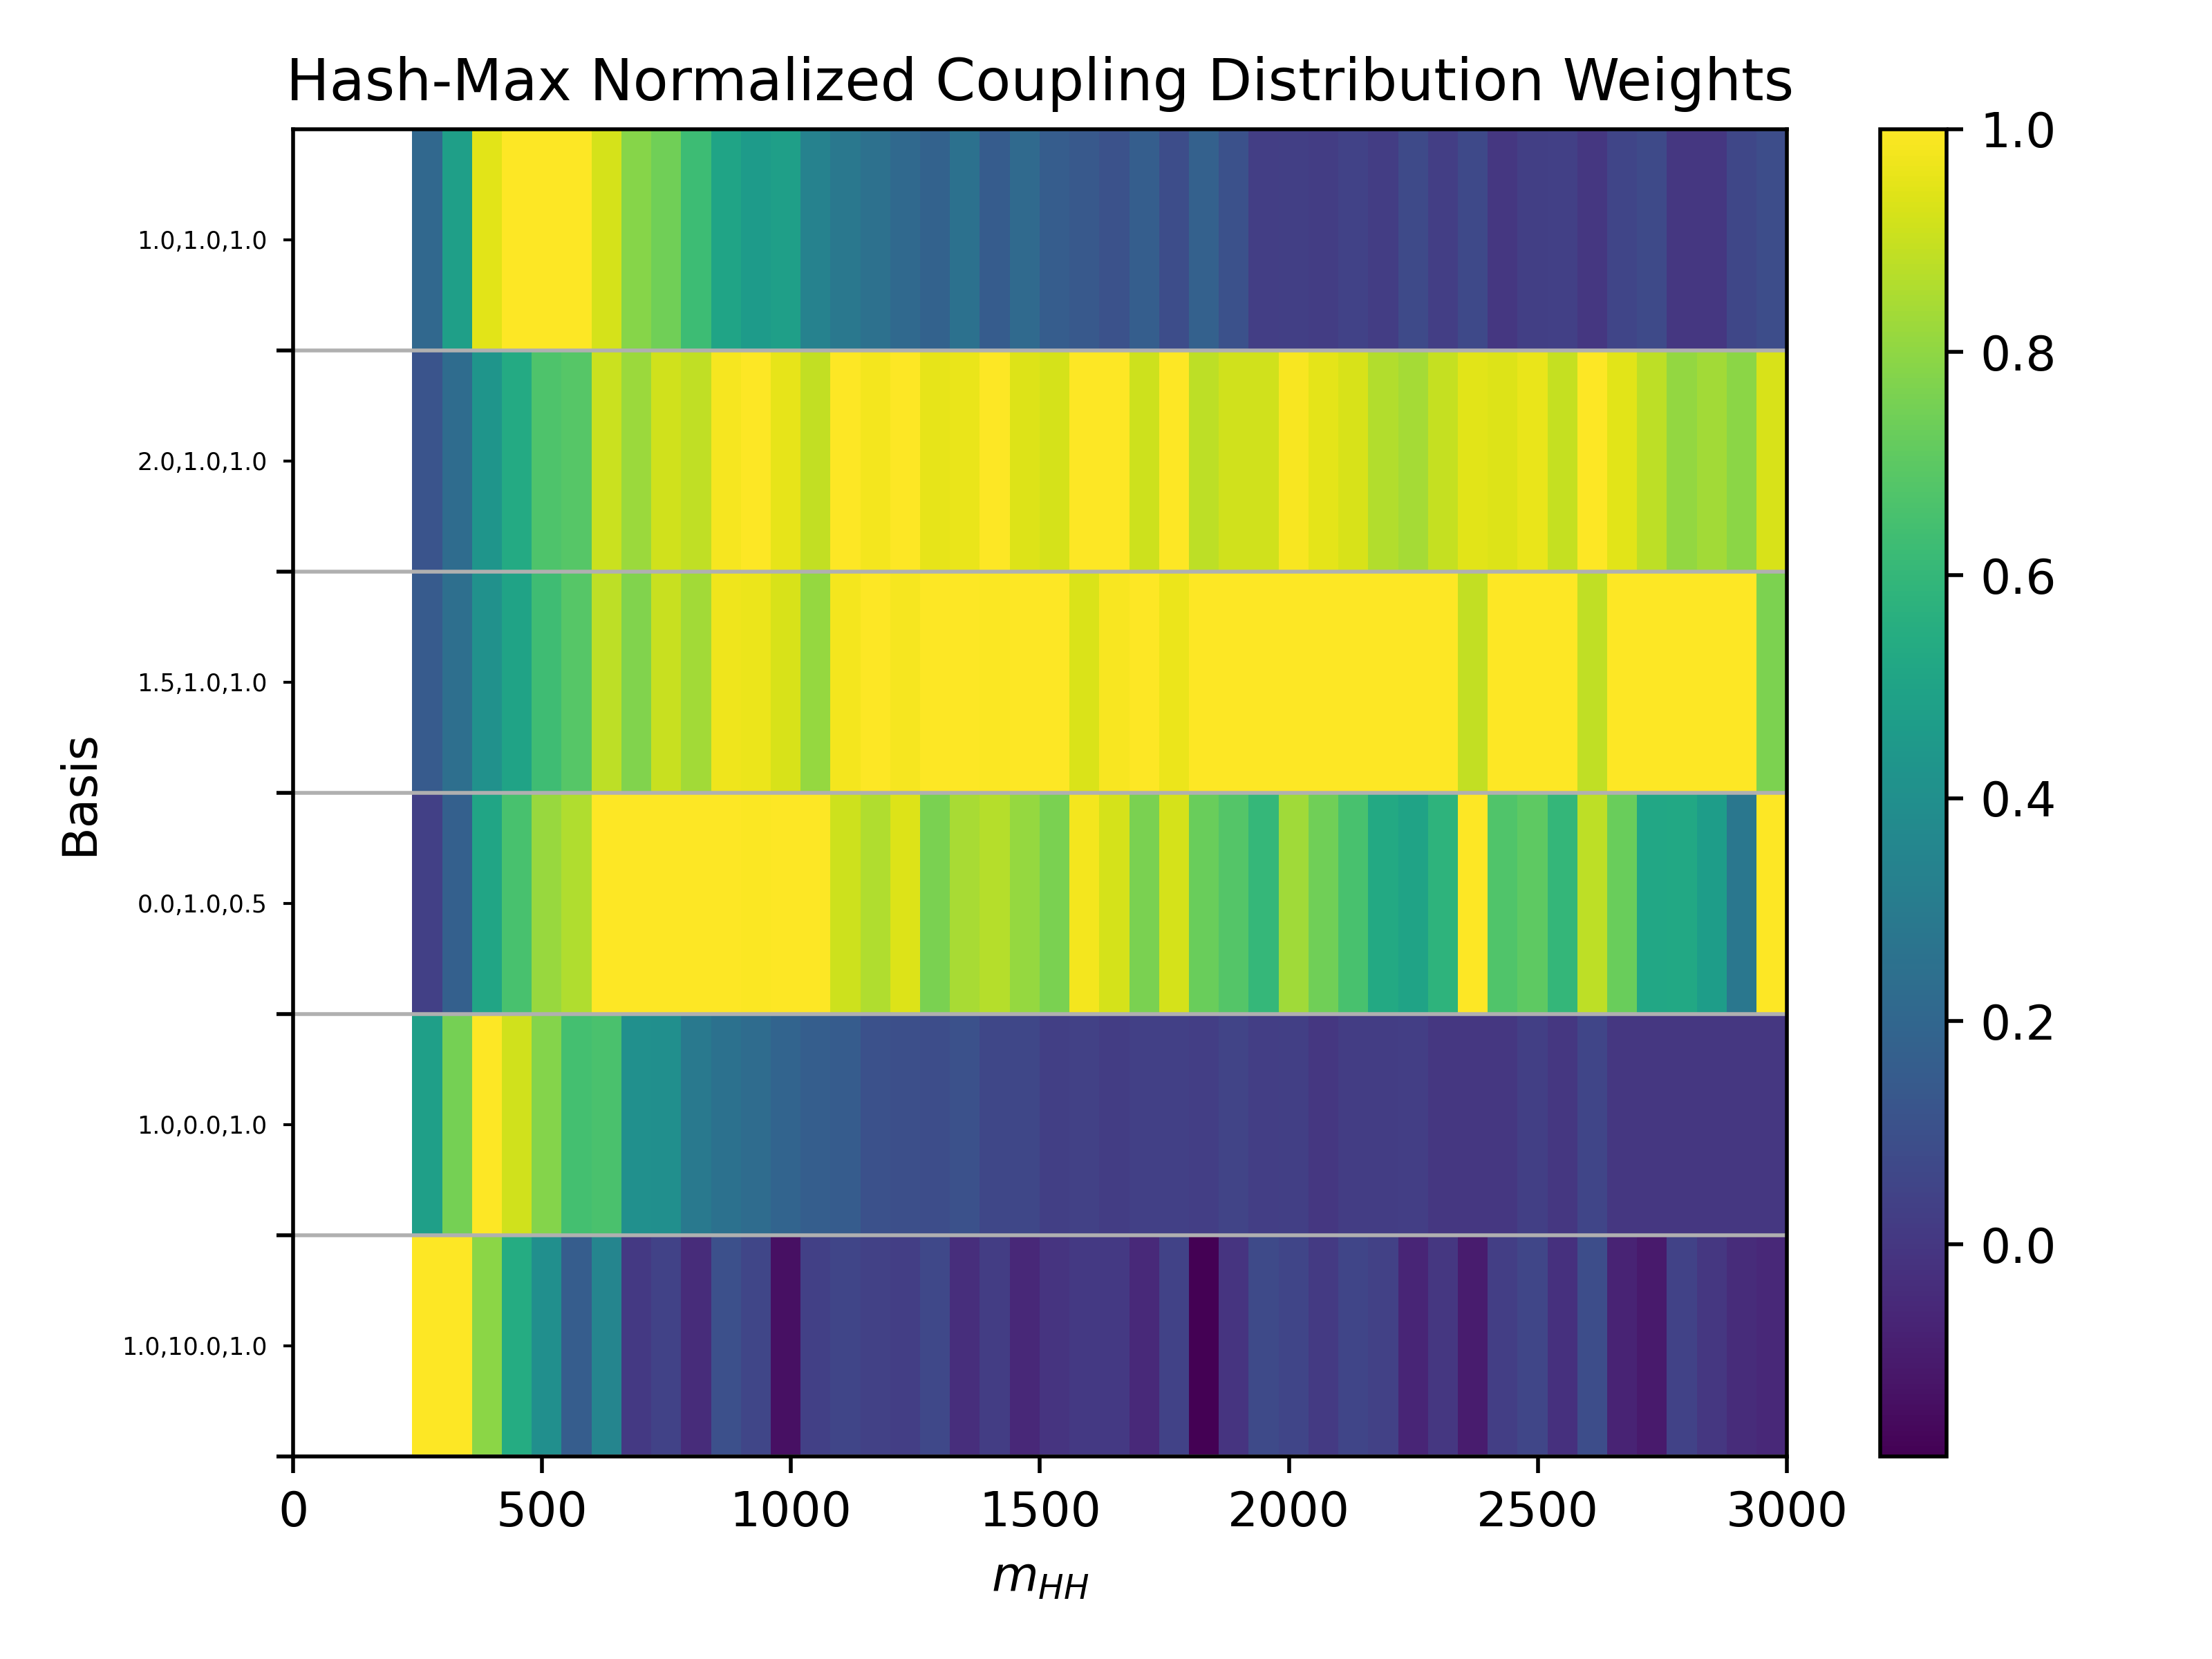
\includegraphics[width=\linewidth,height=\textheight,keepaspectratio]
            {coupling_scan_auto_chosen_reco_R0_hash_max}

        \end{column}
        \begin{column}{0.6\textwidth}
            \resizebox{0.8\textwidth}{!}{ \begin{minipage}{1.0\textwidth}
            Linear Combination Equation

            \vspace{10mm}

            {\tiny $
    \left(2 \kappa_{2V}^{2} - \frac{124 \kappa_{2V} \kappa_{V}^{2}}{9} + \frac{61 \kappa_{2V} \kappa_{V} \kappa_{\lambda}}{9} + \frac{106 \kappa_{V}^{4}}{9} - \frac{17 \kappa_{V}^{3} \kappa_{\lambda}}{3} - \frac{\kappa_{V}^{2} \kappa_{\lambda}^{2}}{9}\right) \left|{A{\left(1,1,1 \right)}}\right|^{2} +
$

$
    \left(2 \kappa_{2V}^{2} - 8 \kappa_{2V} \kappa_{V}^{2} + 3 \kappa_{2V} \kappa_{V} \kappa_{\lambda} + 6 \kappa_{V}^{4} - 3 \kappa_{V}^{3} \kappa_{\lambda}\right) \left|{A{\left(2,1,1 \right)}}\right|^{2} +
$

$
    \left(- 4 \kappa_{2V}^{2} + 20 \kappa_{2V} \kappa_{V}^{2} - 8 \kappa_{2V} \kappa_{V} \kappa_{\lambda} - 16 \kappa_{V}^{4} + 8 \kappa_{V}^{3} \kappa_{\lambda}\right) \left|{A{\left(1.5,1,1 \right)}}\right|^{2} +
$

$
    \left(16 \kappa_{2V} \kappa_{V}^{2} - 16 \kappa_{2V} \kappa_{V} \kappa_{\lambda} - 16 \kappa_{V}^{4} + 16 \kappa_{V}^{3} \kappa_{\lambda}\right) \left|{A{\left(0,1,0.5 \right)}}\right|^{2} +
$

$
    \left(\frac{4 \kappa_{2V} \kappa_{V}^{2}}{5} - \frac{4 \kappa_{2V} \kappa_{V} \kappa_{\lambda}}{5} + \frac{\kappa_{V}^{4}}{5} - \frac{3 \kappa_{V}^{3} \kappa_{\lambda}}{10} + \frac{\kappa_{V}^{2} \kappa_{\lambda}^{2}}{10}\right) \left|{A{\left(1,0,1 \right)}}\right|^{2} +
$

$
    \left(- \frac{\kappa_{2V} \kappa_{V}^{2}}{45} + \frac{\kappa_{2V} \kappa_{V} \kappa_{\lambda}}{45} + \frac{\kappa_{V}^{4}}{45} - \frac{\kappa_{V}^{3} \kappa_{\lambda}}{30} + \frac{\kappa_{V}^{2} \kappa_{\lambda}^{2}}{90}\right) \left|{A{\left(1,10,1 \right)}}\right|^{2}
$
}
            \end{minipage}}
        \end{column}
    \end{columns}
}
\frame{
    \frametitle{New VBF Samples Will be Available Shortly}
    \begin{columns} \begin{column}{0.5\textwidth}
        \begin{center} 
        Current MC Samples

        (70 Possible Combinations of 6)

        \resizebox{0.3\textheight}{!}{\begin{tabular}{ |l|l|l| }
            \hline
            \textbf {$\kappa_{2V}$} & \textbf {$\kappa_\lambda$} & \textbf {$\kappa_V$} \\
            \hline
 \rowcolor{red}   0   & 0   & 1   \\ % !!
                  0   & 1   & 1   \\ 
                  0.5 & 1   & 1   \\ 
                  1   & 0   & 1   \\ 
 \rowcolor{red}   1   & 1   & 0.5 \\ % !!
                  1   & 1   & 1   \\ 
 \rowcolor{red}   1   & 1   & 1.5 \\ % !!
                  1   & 10  & 1   \\ 
                  1   & 2   & 1   \\ 
                  1.5 & 1   & 1   \\ 
                  2   & 1   & 1   \\ 
                  4   & 1   & 1   \\ 
 \rowcolor{green} 0   & 1   & 0.5 \\ % !!
            \hline
        \end{tabular}} \end{center}
    \end{column} \begin{column}{0.5\textwidth}
        \begin{center}

        New MC Samples

        (619 Possible Combinations of 6)

        \resizebox{0.3\textheight}{!}{\begin{tabular}{ |l|l|l| }
            \hline
            \textbf {$\kappa_{2V}$} & \textbf {$\kappa_\lambda$} & \textbf {$\kappa_V$} \\
            \hline
            0    & 0   & 1   \\
            0    & 1   & 1   \\
            0.5  & 1   & 1   \\
            1    & 0   & 1   \\
            1    & 1   & 0.5 \\
            1    & 1   & 1   \\
            1    & 1   & 1.5 \\
            1    & 10  & 1   \\
            1    & 2   & 1   \\
            1.5  & 1   & 1   \\
            2    & 1   & 1   \\
            3    & 1   & 1   \\
            \hline
        \end{tabular}} \end{center}
    \end{column} \end{columns}
}


\displayone{Assessing Basis Performance}{
        Original thinking was that

        orthogonal basis = good

        \vspace{5mm}
        However, the statistics involved in combining samples is non-trivial, and I'm less confident in this as an approach.

        \vspace{5mm}
        To start, let's try looking at statistical error more directly...
}{coupling_scan_auto_chosen_reco_R0_hash_max}


\displaythree{Visualizing Error}
{ \small 
    $\kvv$, $\kl$, $m_{HH}$ bins, and relative error for each bin forms a 4D parameter space.
    This is unreasonable to visualize.

    \vspace{5mm}

    Need to trim down dimenionality by focussing on most relevant aspect of parameter space.
    My thinking: Look at the peak of the distribution.

}
{reco_mHH_cvv1p0cl2p0cv1p0}
{reco_mHH_cvv0p0cl1p0cv1p0}
{reco_mHH_cvv4p0cl1p0cv1p0}

\fullscreenimage{$m_{HH}$ Distribution Mode Across $\kvv$-$\kl$ $(\kv=1)$ Space}{combination_grid_mode}

\displaytwo{Modal Relative Error Across $\kvv$-$\kl$ Space}
{Errors in the ``diagonal" regions are quite large. Does this matter?}
{combination_grid_mode}{combination_grid_error}

\fullscreenimage{Recall 2D Limits}{2D_scan_scan_test_beta5_samps_vbf_pd_161718_c1v1.0_exclusion}
\fullscreenimage{Trying to Make Sense of Things...}{combination_grid_all}


    \section{Conclusion}
    \displayonelarge{Conclusion}{
        \tiny
        \begin{itemize} {
            \item VBF truth reweighting has been put on indefinite hold in favor of direct combination
            \item New VBF signal samples will soon be available, allowing many different basis possibilities
            \item Focus is now on optimizing selection of a basis set
            \item Currently trying to find a method of visualizing and assessing performance of a given basis
        } \end{itemize}
    }{combination_grid_all}

    \announcesection{Backup}
    \frame{
    \frametitle{Validity of Linear Combinations at Truth-Level}
    \begin{columns}
        \begin{column}{0.4\textwidth}
            \begin{center} 
            {\tiny Basis Set}

            \resizebox{0.2\textheight}{!}{\begin{tabular}{ |l|l|l| }
                \hline
                \textbf {$\kappa_{2V}$} & \textbf {$\kappa_\lambda$} & \textbf {$\kappa_V$} \\
                \hline
                1.  &  1. &  1.  \\
                1.5 &  1. &  1.  \\
                2.  &  1. &  1.  \\
                1.  &  0. &  1.  \\
                1.  & 10. &  1.  \\
                1.  &  1. &  1.5 \\
                \hline
            \end{tabular}} \end{center}

            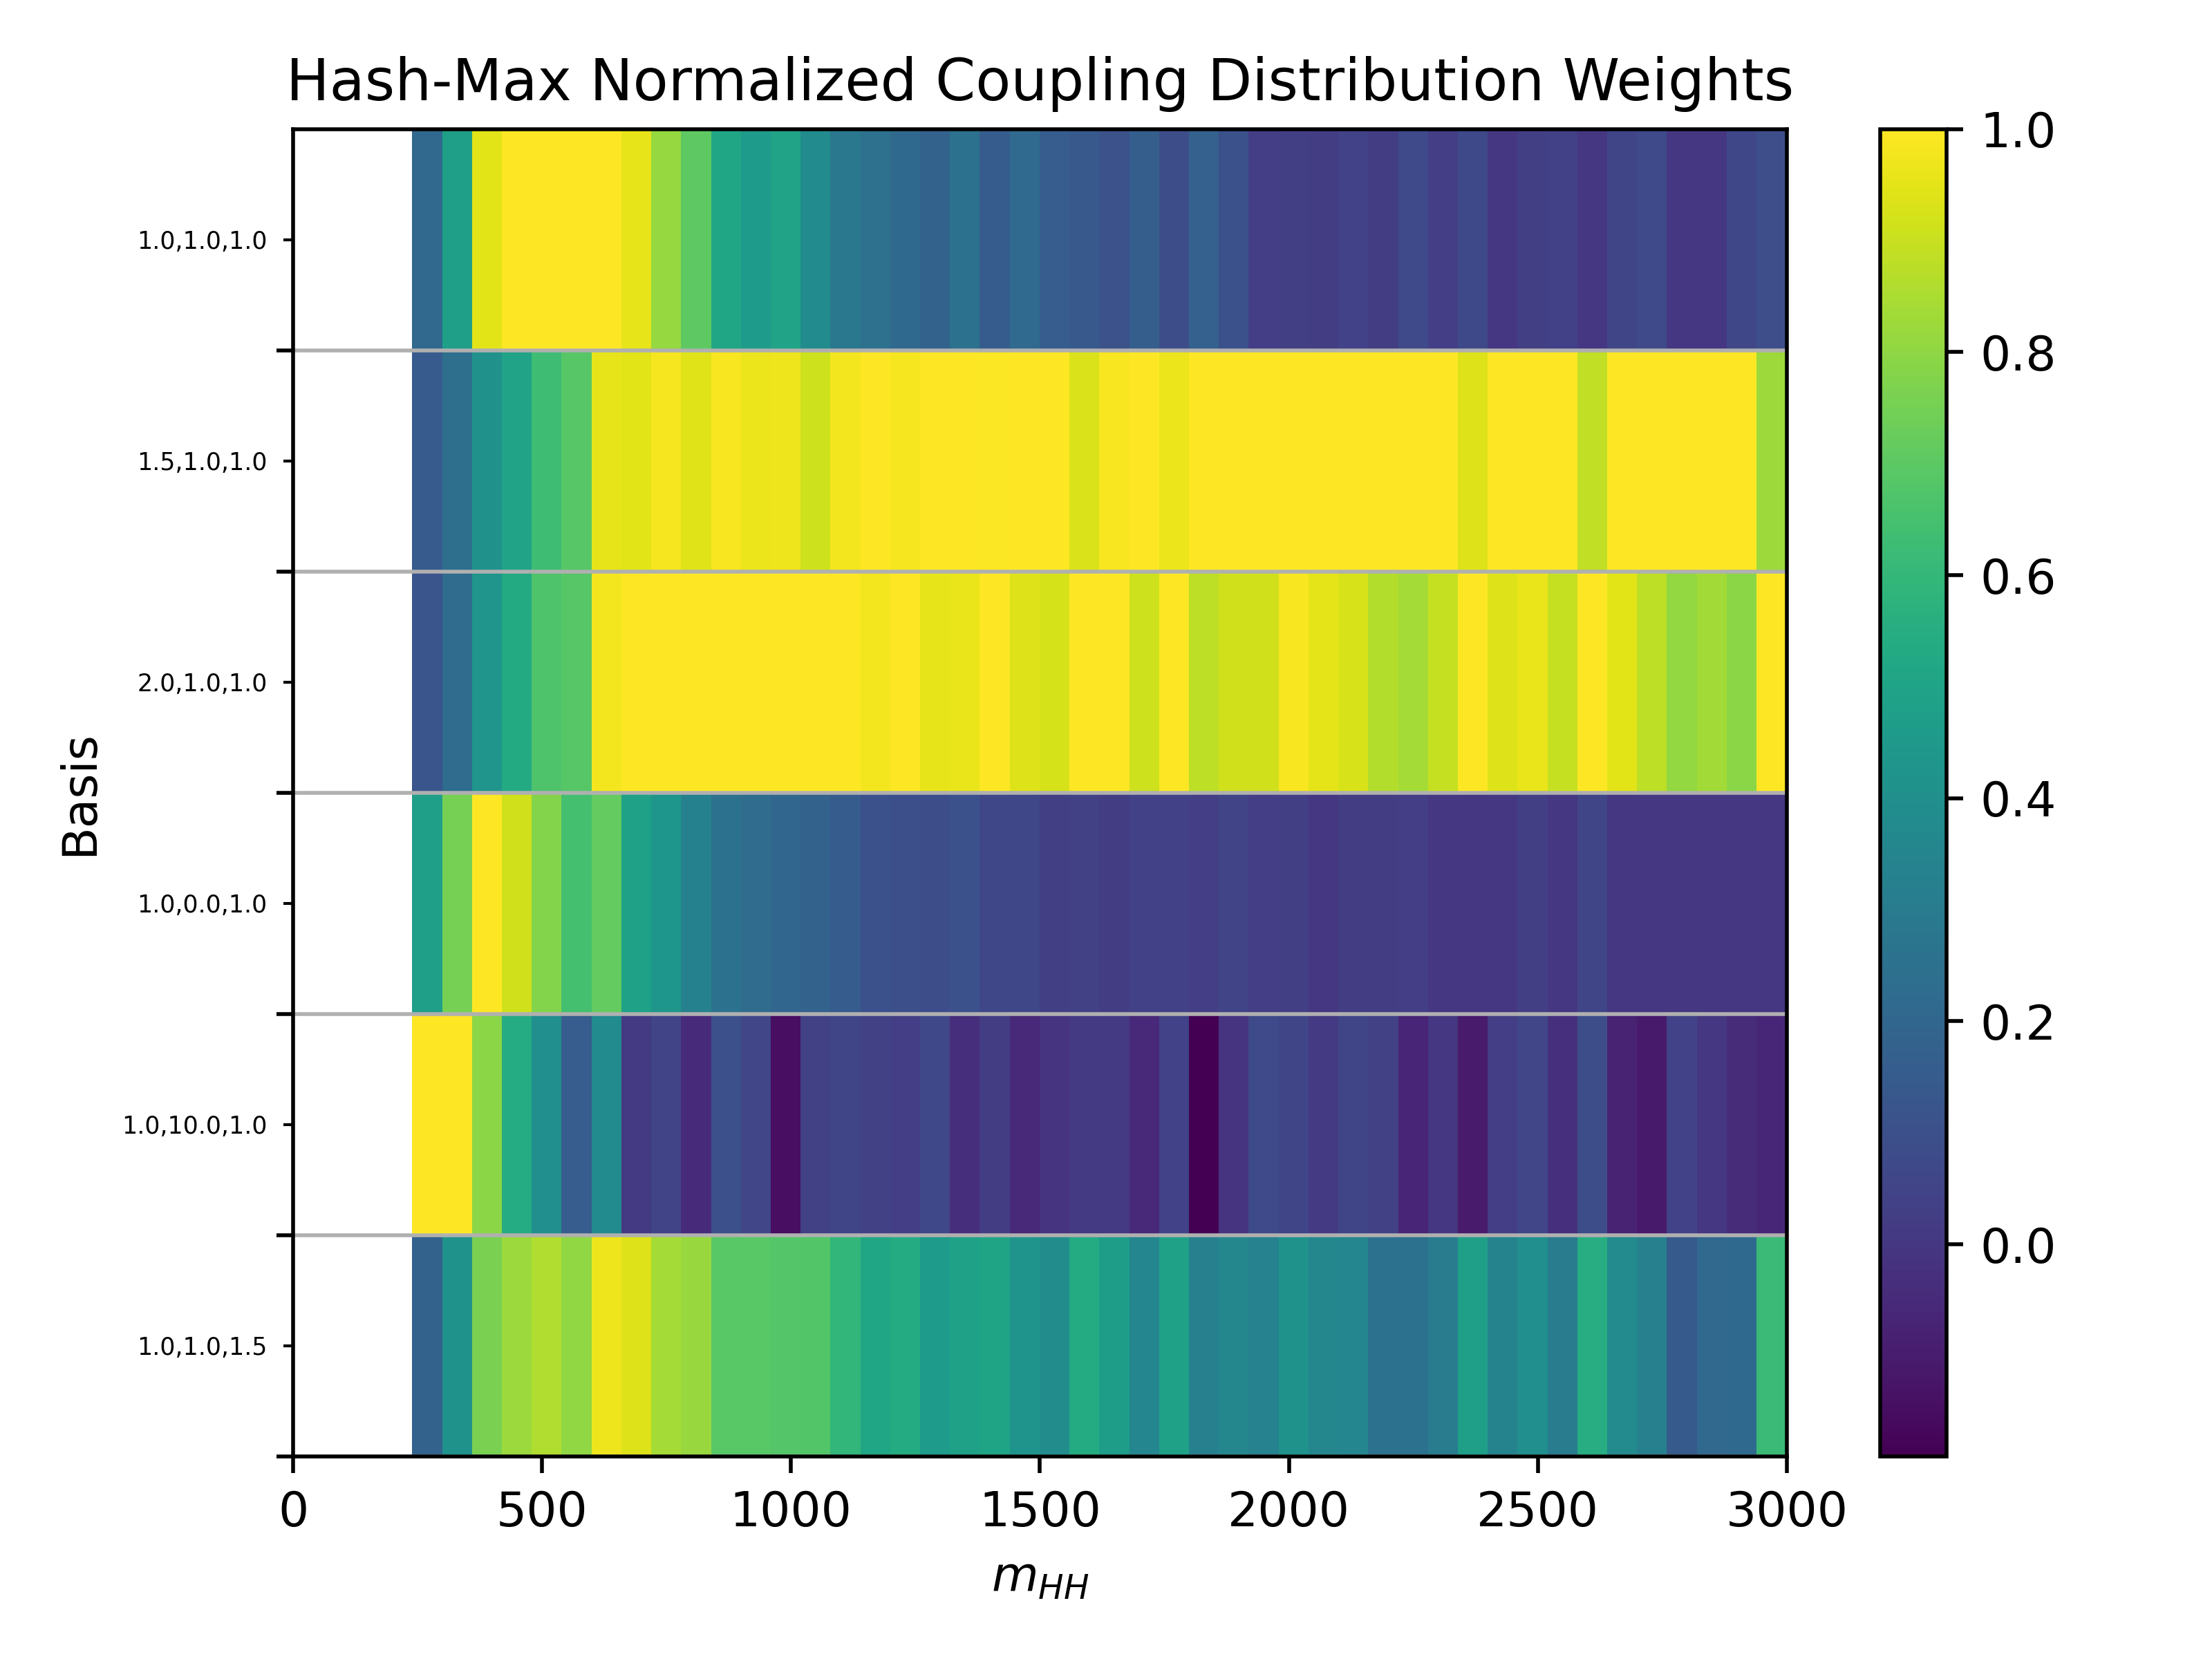
\includegraphics[width=\linewidth,height=\textheight,keepaspectratio]
                {coupling_scan_auto_chosenR1_hash_max}

        \end{column}
        \begin{column}{0.6\textwidth}
            \resizebox{0.8\textwidth}{!}{ \begin{minipage}{1.0\textwidth}
            Linear Combination Equation

            \vspace{10mm}

            {\tiny $
\left|{A{\left(1,1,1 \right)}}\right|^{2} \left(2 \kappa_{2V}^{2} + \frac{136 \kappa_{2V} \kappa_{V}^{2}}{15} - \frac{241 \kappa_{2V} \kappa_{V} \kappa_{\lambda}}{15} - \frac{166 \kappa_{V}^{4}}{15} + \frac{773 \kappa_{V}^{3} \kappa_{\lambda}}{45} - \frac{\kappa_{V}^{2} \kappa_{\lambda}^{2}}{9}\right)
+ \left|{A{\left(1.5,1,1 \right)}}\right|^{2}  \left(- 4 \kappa_{2V}^{2} - \frac{20 \kappa_{2V} \kappa_{V}^{2}}{3} + \frac{56 \kappa_{2V} \kappa_{V} \kappa_{\lambda}}{3} + \frac{32 \kappa_{V}^{4}}{3} - \frac{56 \kappa_{V}^{3} \kappa_{\lambda}}{3}\right)
+ \left|{A{\left(2,1,1 \right)}}\right|^{2} \left(2 \kappa_{2V}^{2} + \frac{4 \kappa_{2V} \kappa_{V}^{2}}{3} - \frac{19 \kappa_{2V} \kappa_{V} \kappa_{\lambda}}{3} - \frac{10 \kappa_{V}^{4}}{3} + \frac{19 \kappa_{V}^{3} \kappa_{\lambda}}{3}\right)
+ \left|{A{\left(1,0,1 \right)}}\right|^{2} \left(\frac{42 \kappa_{2V} \kappa_{V}^{2}}{25} - \frac{42 \kappa_{2V} \kappa_{V} \kappa_{\lambda}}{25} - \frac{17 \kappa_{V}^{4}}{25} + \frac{29 \kappa_{V}^{3} \kappa_{\lambda}}{50} + \frac{\kappa_{V}^{2} \kappa_{\lambda}^{2}}{10}\right)
+ \left|{A{\left(1,10,1 \right)}}\right|^{2} \left(- \frac{\kappa_{2V} \kappa_{V}^{2}}{75} + \frac{\kappa_{2V} \kappa_{V} \kappa_{\lambda}}{75} + \frac{\kappa_{V}^{4}}{75} - \frac{11 \kappa_{V}^{3} \kappa_{\lambda}}{450} + \frac{\kappa_{V}^{2} \kappa_{\lambda}^{2}}{90}\right) 
+ \left|{A{\left(1,1,1.5 \right)}}\right|^{2} \left(- \frac{16 \kappa_{2V} \kappa_{V}^{2}}{15} + \frac{16 \kappa_{2V} \kappa_{V} \kappa_{\lambda}}{15} + \frac{16 \kappa_{V}^{4}}{15} - \frac{16 \kappa_{V}^{3} \kappa_{\lambda}}{15}\right)
$
}
            \end{minipage}}
        \end{column}
    \end{columns}
}

\displaythree{Truth Combination Plots}
{Note that variation (1,1,1) is among the basis states and only present as a sanity check.}
{truth_comb_cvv1p0cl1p0cv1p0}
{truth_comb_cvv1p0cl20p0cv1p0}
{truth_comb_cvv1p0cl1p0cv0p5}
 
\displaythree{More Truth Combination Plots}{}
{truth_comb_cvv0p0cl0p0cv1p0}
{truth_comb_cvv0p0cl1p0cv1p0}
{truth_comb_cvv0p5cl1p0cv1p0}
 
\displaythree{Yet More Truth Combination Plots}{}
{truth_comb_cvv1p0cl2p0cv1p0}
{truth_comb_cvv1p0cl5p0cv1p0}
{truth_comb_cvv3p0cl1p0cv1p0}



\end{document}
